\documentclass[tikz,border=8pt]{standalone}
\usepackage{amsmath}
\usetikzlibrary{arrows.meta,calc}
\definecolor{ink}{HTML}{21352F}
\definecolor{teal}{HTML}{087F7B}
\definecolor{blue}{HTML}{4B77A8}
\definecolor{gold}{HTML}{C58B2A}
\definecolor{rose}{HTML}{B65A62}
\begin{document}
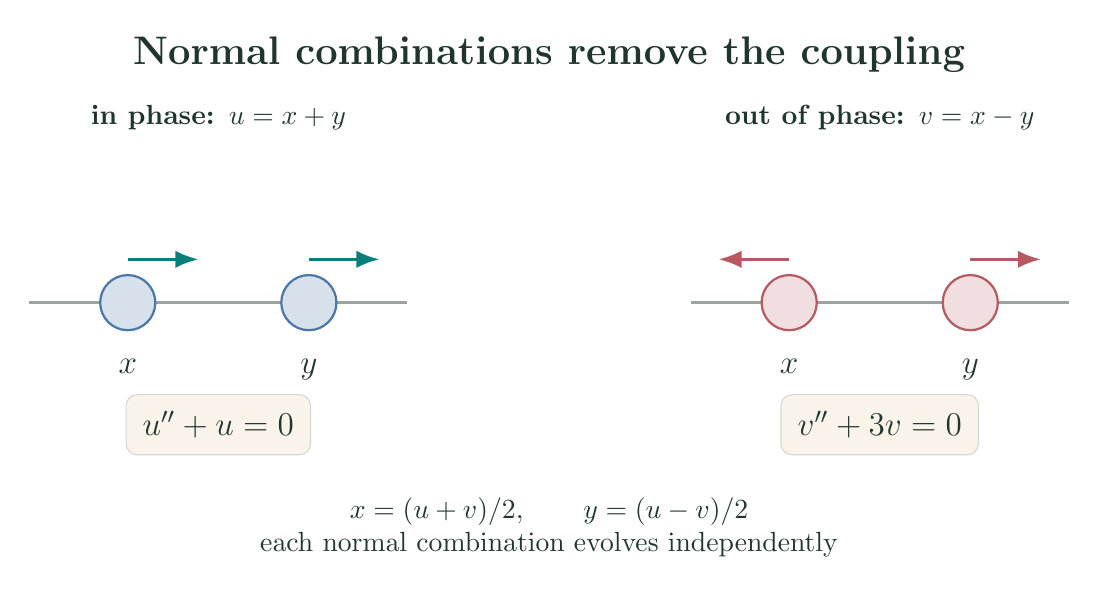
\begin{tikzpicture}[font=\large\sffamily,text=ink,>=Latex]
  \node[font=\bfseries\Large] at (0,3.15)
    {Normal combinations remove the coupling};

  \begin{scope}[xshift=-4.2cm]
    \node[font=\bfseries] at (0,2.35) {in phase: $u=x+y$};
    \draw[ink!45,very thick] (-2.4,0)--(2.4,0);
    \fill[blue!22,draw=blue,thick] (-1.15,0) circle (.35);
    \fill[blue!22,draw=blue,thick] (1.15,0) circle (.35);
    \draw[teal,very thick,->] (-1.15,.55)--(-.25,.55);
    \draw[teal,very thick,->] (1.15,.55)--(2.05,.55);
    \node[below=7pt] at (-1.15,-.35) {$x$};
    \node[below=7pt] at (1.15,-.35) {$y$};
    \node[draw=ink!20,fill=gold!10,rounded corners=4pt,inner sep=6pt]
      at (0,-1.55) {$u''+u=0$};
  \end{scope}

  \begin{scope}[xshift=4.2cm]
    \node[font=\bfseries] at (0,2.35) {out of phase: $v=x-y$};
    \draw[ink!45,very thick] (-2.4,0)--(2.4,0);
    \fill[rose!20,draw=rose,thick] (-1.15,0) circle (.35);
    \fill[rose!20,draw=rose,thick] (1.15,0) circle (.35);
    \draw[rose,very thick,->] (-1.15,.55)--(-2.05,.55);
    \draw[rose,very thick,->] (1.15,.55)--(2.05,.55);
    \node[below=7pt] at (-1.15,-.35) {$x$};
    \node[below=7pt] at (1.15,-.35) {$y$};
    \node[draw=ink!20,fill=gold!10,rounded corners=4pt,inner sep=6pt]
      at (0,-1.55) {$v''+3v=0$};
  \end{scope}

  \node[align=center,font=\normalsize] at (0,-2.85)
    {$x=(u+v)/2,\qquad y=(u-v)/2$\\
     each normal combination evolves independently};
\end{tikzpicture}
\end{document}
